\documentclass{standalone}

\usepackage{tikz}
\usetikzlibrary{mindmap,trees}
\usepackage{verbatim}

\begin{document}
\pagestyle{empty}

\begin{comment}

\end{comment}

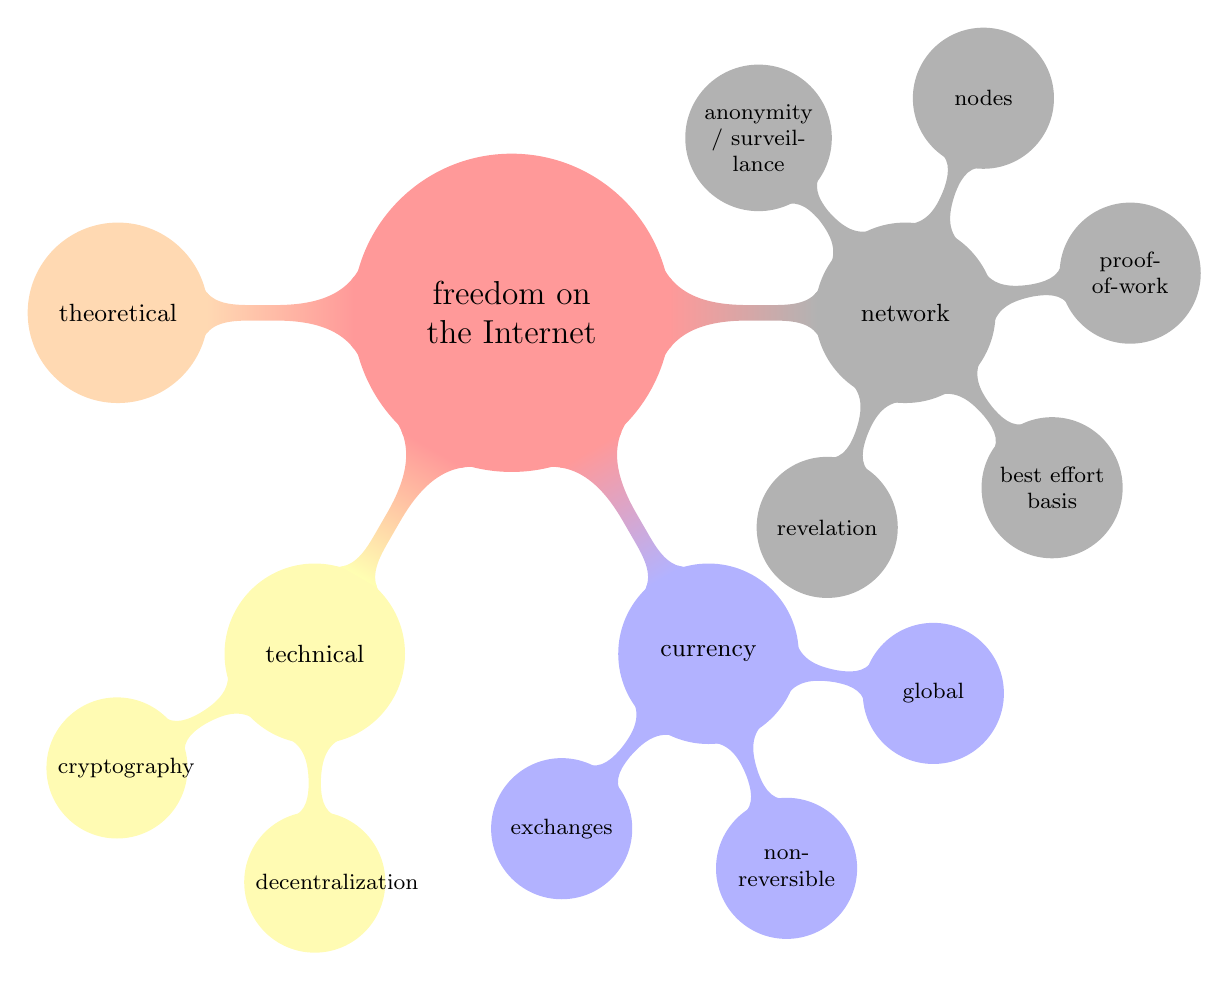
\begin{tikzpicture}
	\path[mindmap,concept color=red!40!white,text=black]
		node[concept] {freedom on the Internet}
		[clockwise from=0]
		child[concept color=black!30!white] {
			node[concept] {network}
			[clockwise from=130]
			child {
				node[concept] {anonymity / surveillance}
			}
			child {
				node[concept] {nodes}
			}
			child {
				node[concept] {proof-of-work}
			}
			child {
				node[concept] {best effort basis}
			}
			child {
				node[concept] {revelation}
			}
		}  
		child[concept color=blue!30!white] {
			node[concept] {currency}
			[clockwise from=-10]
			child {
				node[concept] {global}
			}
			child {
				node[concept] {non-reversible}
			}
			child {
				node[concept] {exchanges}
			}
		}
		child[concept color=yellow!30!white] {
			node[concept] {technical}
			[clockwise from=-90]
			child {
				node[concept] {decentralization}
			}
			child {
				node[concept] {cryptography}
			}
		}
		child[concept color=orange!30!white] {
			node[concept] {theoretical}
		};
\end{tikzpicture}\end{document}
